\documentclass[11pt]{article}
\usepackage{latexsym}
\usepackage{amsmath}
\usepackage{amssymb}
\usepackage{amsthm}
\usepackage{epsfig}
\usepackage{psfig}
\usepackage{url}
\usepackage{algorithm}
\usepackage{algorithmic}
% \usepackage[pdftex]{graphicx}
\usepackage{subfig}
\usepackage{color}
\usepackage{xcolor}
\usepackage{listings}

\usepackage{caption}
\DeclareCaptionFont{white}{\color{white}}
\DeclareCaptionFormat{listing}{\colorbox{gray}{\parbox{\textwidth}{#1#2#3}}}
\captionsetup[lstlisting]{format=listing,labelfont=white,textfont=white}




% 1-inch margins, from fullpage.sty by H.Partl, Version 2, Dec. 15, 1988.
\topmargin 0pt \advance \topmargin by -\headheight \advance \topmargin by
-\headsep \textheight 8.9in \oddsidemargin 0pt \evensidemargin \oddsidemargin
\marginparwidth 0.5in \textwidth 6.5in

\parindent 0in \parskip 1.5ex
% \renewcommand{\baselinestretch}{1.25}

\begin{document}

\title{Truthfulness Verification System}

\author{
Tathagata Dasgupta, ABM Musa\\
Email: \{tdasgu2, amusa2\}@uic.edu\\
URL: http://code.google.com/p/tverifier }

\date{}
\maketitle


\section{Introduction}
Web has became the most prevalent source of information now a days. However, many
information on the web is untruthful. Also because of the widespread reach of
web, sometimes web is used to propagate untruthful facts for social and political
reasons. Hence with the increasingly use of web as information source,
verification of information truthfulness became an important facet to consider.

The popular search engines extract information from web based on keywords and
metadata without considering the truthfulness of the facts. Also, there have been
not much research in this area. To our best knowledge, the most recent work on this area is T-verifier  \cite{tverifier}, which uses results from search engines
to verify truthfulness of statements. T-verifier performs very well on the
test-dataset. However, T-verifier has some problems with the overall approach to
verify the truthfulness of statements and there is room for improvement. In this
work, we will extend the T-verifier system so that it's weaknesses can be
resolved to get a more robust truthfulness verification system.


\section{Current System}
Current system for truthfulness verification is called T-verifier
\cite{tverifier}, which uses two phase methods for truthfulness verification of
statements. Each of these two phases rely heavily on search results returned by
popular search engines. T-verifier takes the doubtful statements (DS) as input
from the user along with the doubtful unit (DU). Phrase after removing DU from DS
is called topic unit (TU).

At the first phase, T-verifier generates alternative statements by supplying
$TU$ to search engine and collecting the relevant alternate $DU$-s. However,
from basic web search may result in lot of alternate DUs that are not semantically or
logically relevant to the original DS. Hence, T-verifier uses combination of
seven features to rank alternate DUs. These features primarily exploit the facts
that relevant alternative units frequently co-occur, people often mention both
misconception and truthful conception together, data-type matching, and
sense-closeness. T-verifier chooses top 5 alternative statements based on top 5
alternate DUs obtained in this phase.

At the second phase, top 5 alternative statements from phase 1 is supplied to the
search engine again. Then the returned searched result is ranked by multiple
rankers such as Alternative Unit Ranker, Hits ranker, Text-feature Ranker, Domain
Authority Ranker etc. Then all those ranks are merged to form an overall ranking
among the alternate statements and top statement in this final merged ranking is
considered as truthful statement.

% We are currently working to get the T-verifier code running on our systems,
% with inputs from Xian Li. So the descriptions below lacks some required details
% and makes some assumptions.   As of now T-Verifier produces 5 alternative
% statements once it is provided with a doubtful statement (DS), a doubtful unit
% (DU), data type of the unit etc in the first phase. Though these sentences
% produced are quite accurate, the facility to pinpoint the correct alternative
% does exist yet. The project goal, may be formulated as:  "Extract information
% from Wikipedia and ontologies ( such as Yago, DBpedia and Freebase) which helps
% to verify truthfulness of statements. Describe the extraction algorithm and how
% the information can be utilized to assist statement truthfulness verification."

\section{Problems with Current System}
Although results from the tested dataset achieves good performance (90\%
accuracy), failing of T-verifier for some statements shows that it has some
inherent problems and there is room for improvement.

First, T-verifier assumes that truthful statements will be more propagated in the
web compared to the untruthful statement. However, this may be not true in
general because of intended and planned propaganda for establishing some
untruthful statements. This kind of propagandas are even becoming more common now
a days due to widespread reach of Internet. T-verifier also showed that \emph{"Hillary
Clinton is the President of United States"} has more hits than \emph{"Hillary Clinton is
the Secretary of State"}. Although T-verifier was able to find the correct
statement in this case using multiple ranks together, in general the untruthful
statement can be prevalent in the web compared to truthful statements.

Second, T-verifier do not use the reputation of the information source.
T-verifier uses only search results returned by the search engine irrespective of
the origin and believability of the information origin. Hence there is room for
improvement here to give more weight to the information obtained from trustworthy
sources such as Wikipedia.


\section {Propsed System}


\begin{figure}
  \centering
  \subfloat[System
  overview]{\label{fig:System}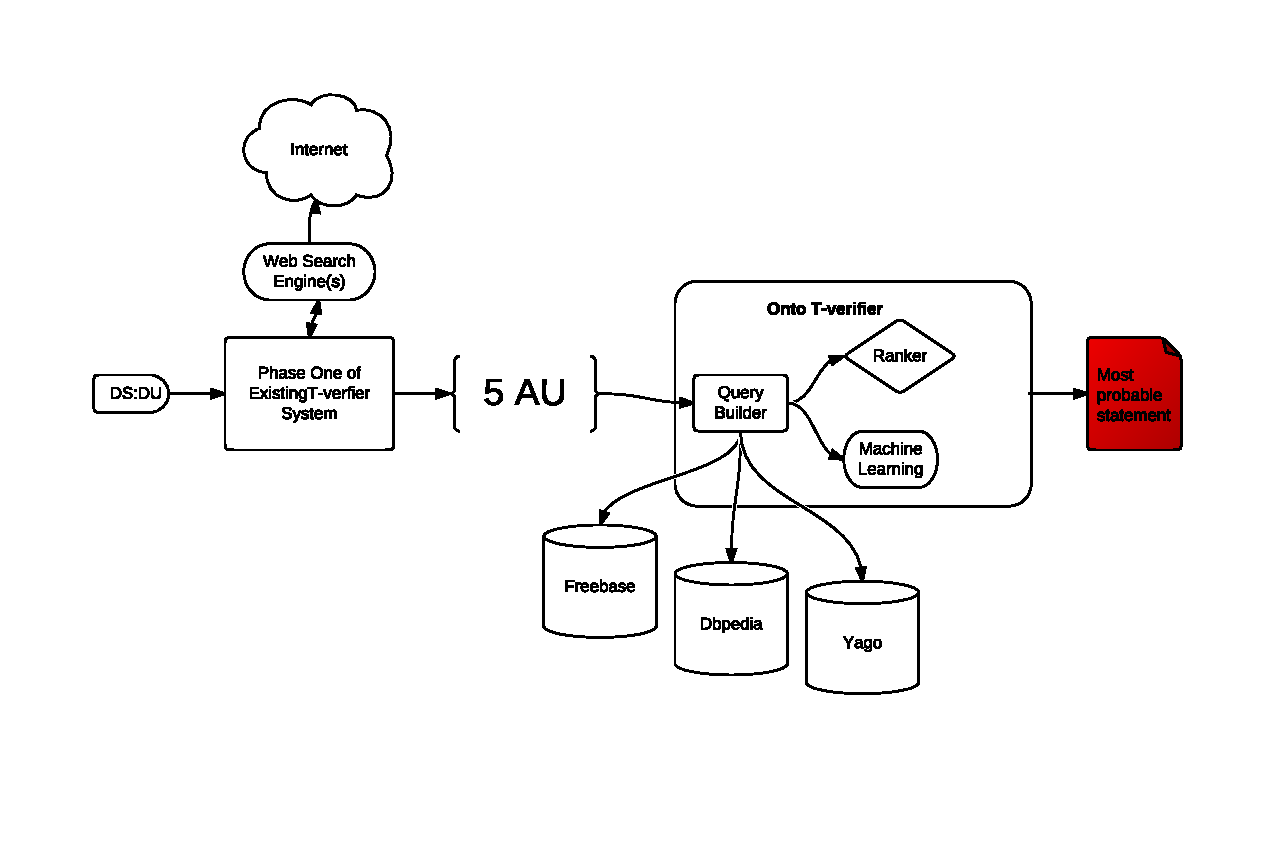
\includegraphics[width=0.85\textwidth]{system.pdf}}
  \caption{System overview}
  \label{fig:system}
\end{figure}


\subsection{Description of extraction algorithm}

For disambiguation among the alternative statements, Wikipedia is generally used
as an authoritative source. However, the contents of Wikipedia is not available
in the form that is consumable in a programmatic format. To address such
difficulties a number of projects Yago, DBpedia, Freebase have organized the
massive amount of data in a searchable fashion e.g DBpedia uses SPARQL endpoint,
Freebase uses MQL api. Open source implementation of Python wrappers exist for
both the interfaces exist and appear to be mature enough for our needs.

\subsubsection{Freebase} 
Freebase has information about approximately 20 million Topics, each one having a
unique Id, which can help distinguish multiple entities which have similar names,
such as Henry Ford the industrialist vs Henry Ford the footballer. Most of the
topics are associated with one or more types\cite{freebasetype} (such as
people, places, books, films, etc) and may have additional properties like "date of birth" for a person
or latitude and longitude for a location. Freebase not only contains data from
the Wikipedia but also other sources; users can submit data to the Freebase
datastore and expand it in richness. We tinkered with the api\cite{freebaseapi}
and it appeared to be the most viable starting point for the project.

\subparagraph{Motivational Example}

\begin{lstlisting}[label=some-code,caption=Minimal code to Freebase]

import freebase
import pprint

query = [{
  "a:starring": [{
    "actor": "Meg Ryan"                                                       
  }],
  "b:starring": [{                                                            
    "actor": "Tom Hanks"
  }],
  "type": "/film/film",
  "*": [],
}]  
    
pp = pprint.PrettyPrinter(indent=4)
result = freebase.mqlread(query)
    
print "Movie names & their various forms"
    
    
for i in result:                                                              
        pp.pprint(i["key"])                                                   
                
\end{lstlisting}
\begin{lstlisting}[label=output,caption=Cleaned Output]

Movie names & their various forms
[   '158982',
    'You$0027ve_Got_Mail',
    '18171032',

     ...
    'E-m$0040il_f$00FCr_Dich',
    'youve-got-mail']
[   '176489',
    'Joe_Versus_the_Volcano',
    'Joe_Vs$002E_The_Volcano',
    'Brain_Cloud',
     ...
    '2327353',
    'joe-versus-the-volcano']
[   '226198',
    'Sleepless_in_Seattle',
    'Sleepless_In_Seattle',
     ....
    '169146',
    '106482',
    'Insonnia_d$0027amore',
    '62812',
    'Schlaflos_in_Seattle',
    'sleepless-in-seattle'\]

\end{lstlisting}

The above results show how the three movies starring Tom Hanks and Meg Ryan.
When we query Google with Tom Hanks and Meg Ryan, the top result is a page from
Answers.com where a user has asked which are the movies where the two actors
appear together, and the answer lists these three movies namely - ``Joe versus
the Volcano'', `` Sleepless in Seatle'' and ``You\'ve got Mail''. A quick lookup
of the Wikipedia and IMDB pages also confirm the same. 

\subsubsection{Dbpedia}
DBpedia is a similar project to Freebase, but it focuses mainly on the content
available from Wikipedia. It scores in being precisely importing the data from
the info boxes in Wikipedia pages, but at this stage it does not seem to be
offering anything additional over Freebase \cite{freebasedbpedia}. We are yet to
explore its programmatic interface \cite{dbpediaapi}.


\subsubsection{Yago}
YAGO is a semantic knowledge base with over 900,000 entities (like persons,
organizations, cities, etc.) and uses Wikipedia and Wordnet as its main source of
information. We are yet to explore the programmatic interfaces it provides and
how we can use it for the project.




\subsection{Truthfulness verification }
\subsubsection {Building queries from the data supplied by the user}

{\em Wed Mar 9 2011}

Formulating a proper Freebase query is for our specific purpose is a different process than the standard way of querying a search engine that does full text search on text documents. We start by introducing the  various abstraction levels associated with the freebase data.
\begin{itemize}
    \item  A {\em type} is a conceptual container of related {\em properties} commonly needed to describe a certain aspect of a {\em topic}.
    \item  A {\em topic} can be assigned one or more types (the default type being /common/topic)
    \item  As {\em properties} are grouped into {\em types}, {\em types} are grouped into {\em domains}.
    \item  {\em Domains, types}, and {\em properties} are given IDs in a {\em namespace/key} hierarchy.
    \item  Common well-known topics are given IDs in the /en namespace, which are human-readable English strings.
    \item  {\em Topics} are uniquely identified within Freebase by {\em GUIDs}.
    \item  {\em Properties} are {\em multi-value} by default, and multi-value properties and single-value properties can be queried in the same way.
\end{itemize}
In order to transform a sentence to a freebase query we have to one to one map a content word from the sentence($TU$ plus $DU$) to the above mentioned abstraction. In other words, the process involves identifying the contextual meaning of the content words. Although this is pretty intuitive when we do it manually, trying to achieving this programmatically is one the challenging aspect of the project. One way of doing it is using a part of speech taggers, along with chunk extraction and named entity recognition. (details in next section) 

The key point of distinction is that this result set is the set of records from a hierarchical database. We can not stuff in every word from the topic units into a query to freebase, as MQL(metaweb query language) is Query By Example language, and has a rigid structure which is not immediately obvious given a sentence in natural langage. We incrementally build a query $Q$ starting from with one word $w_{i}$ from the word list $L$ extracted from the $TU$. Let the results associated with $q_{w_{i}}$ be ($R_{w_{i}}$). Initially Q = $\{q_{1}=w_{i}\}$

 The following are the possible cases
\begin{itemize}
\item No results - In this case we get the synset from Wordnet $S_{w_{i}}$ and repeat the search with each word in the synseti $w_{j}^{s}$.
\item If there is no match with the word or its synset, we reject $w_{i}$ from the query $Q$ and move on to the next word in $L$ and repeat the process.
\item If $R$ is not empty, we retain the $w_{i}$ or $w_{j}^{s}$ in $Q$. Then we take the each of the remaining words $w_{j}$ from $L$ and $S_{w_{j}}$ and search in $R_{w_{i}}$. If $w_{j}$ or a synonym of it $w_{j}^{s}$ is found to occur in the resulti, we augment $Q$ with $w_{j}$ (or $w_{j}^{s}$). So $Q$ now becomes $Q =\{q_{1}=w_{i}, q_{2}=w_{j}\}$ or $\{q_{1}=w_{i},q_{2}=w_{j}^{s}\}$ 
\item With the new $Q$ we again query Freebase and repeat the above steps.
\item We terminate when all the words (and in their synsets) in $L$ have been substituted. This allows us to form the most appropriate query $Q$ from the $TU$. Note though this is essentially a breadth first search search of the graph, we would not be traversing very deep (though the branching factor can be pretty high) because of the small number of content words in $TU$ and their synsets.
\item If the result returned by this query $Q$ contains the $DU$, we can say with a good degree of confidence that the statement is true.    
\end{itemize}
%\begin{align*}
%q_{i} = \{{TU, AU_{i}, t_{AU_{i}}} \} \qquad \mbox {where $i = 1 \cdots n$} \\
%\end{align*}
%where $n$ is the number of alternative units generated by the first phase of
%the existing system. By quering the various ontologies described above we will
%get results which might have the following cases:
%
%\begin{align*}
%   freebase(q_{i}) &= \phi \\
%    = r_{i}
%\end{align*}
%


\subsection{Examples of Truthfulness Verification}

{\em Wed Mar 9 2011}

\subsubsection{Use of Freebase}

For all the 50 sentences mentioned in the original paper we tried the default POS tagger that comes with the Natural Language toolkit along with NE chunker, Binary NE Chunker and the IEER NE Chunker. None of the yeilded good results. So we used the Illinois named entity extractor from UIUC, which gave comparitively better results primarily because its database is built from various sources like the Wikipedia, Brown Hierarchical Word Clusters etc. 

\begin{itemize}
\item Correctly tagged 19
\item Partly correct 14	
\item Wrong/no identification 12
\end{itemize}



Consider one of the following sentences:

\emph{"Tom Hanks was the lead actress in the movie Sleepless in Seattle"}

Tom/NNP Hanks/NNP was/VBD the/DT lead/NN actress/NN in/IN the/DT movie/NN Sleepless/NNP in/IN Seattle/NNP
Phrases and Named Entities

PERSON:
    Tom/NNP
PERSON:
    Hanks/NNP
GPE:
    Seattle/NNP

Content words for this sentence are "Tom Hanks", "lead", "actress", "movie", "Sleepless in Seattle". 

While "actress" is a domain in freebase, it does not contain anythingi yet. So we look into the synset of the word "actress" from wordnet, which includes \emph{"female actor"}.

Now for the noun phrase \emph{"Sleepless in Seattle"}, we can generate "id" for the query as "sleepless in seattle". But this id will be associated with many properties. To select the relevant property we can use synset obtained from the actress. And this synset has {\em actor}, which is one of the property for id {\em "Sleepless in Seattle"}. Hence the Freebase query can be following:

\begin{lstlisting}


[{
  "id" : "/en/sleepless_in_seattle"
  "/film/film/starring" : [{ "actor" : null }]
}]


Now the result of this query returns following output:

{
  "code":          "/api/status/ok",
  "result": [{
    "/film/film/starring": [
      {
        "actor": "Tom Hanks"
      },
      {
        "actor": "Meg Ryan"
      },
      {
        "actor": "Bill Pullman"
      },
      {
        "actor": "Rosie O'Donnell"
      },
      {
        "actor": "Rob Reiner"
      },
      {
        "actor": "Victor Garber"
      },
      {
        "actor": "Gaby Hoffmann"
      },
      {
        "actor": "Carey Lowell"
      },
      {
        "actor": "David Hyde Pierce"
      },
      {
        "actor": "Ross Malinger"
      },
      {
        "actor": "Frances Conroy"
      },
      {
        "actor": "Rita Wilson"
      }
    ],
    "id": "/en/sleepless_in_seattle"
  }],
  "status":        "200 OK",
  "transaction_id": "cache;cache03.p01.sjc1:8101;2011-03-09T05:09:44Z;0032"
}

\end{lstlisting}

One of the actors in this result set is "Tom Hanks" that matches with our content word "Tom Hanks" in the given sentence. Now as we know earlier that actress means female actor, we can use the keyword female to find the fact that female is type of gender and Freebase id of "tom hanks" has a property gender associated with it. So we can formulate following query.

\begin{lstlisting}

[{
  "id" : "/en/tom_hanks"
  "/people/person/gender" : {}
}]

The result of this query is following:

{
  "code":          "/api/status/ok",
  "result": [{
    "/people/person/gender": {
      "id":   "/en/male",
      "name": "Male",
	.
	.
	.
}	

\end{lstlisting}

Here the gender is Male, which contradicts with our gender female. Hence we can decide that this statement is false. 

For finding the true statement i.e. the actress we can use all actors obtained in the first query result and form second query with their names and output the truthful sentence if we get female as the gender.

\subsubsection{Use of Wikipedia}
Although structured databases such as Freebase, DBPedia extract the information from Wikipedia and format them into a structured and query-friendly way, it does not contain all the relevant information all the time. For example, consider the following sentence:

\emph{Les Paul invented the electric guitar}

The wikipedia page "http://en.wikipedia.org/wiki/Electric\_guitar" contains the inventor of the electric guiter in one of the sentences in the body. But this information is not available in the Freebase. 

We can use a very simple and elegant method to find the relevant information from Wikipedia by using simple web-scrapping and pattern matching using regular expression. The process is described below.

After getting the wikipedia page we can convert the html file into text file and then we can separate all the sentences in different lines. The sentence is the part of the whole text that exist between two full-stops. Another important observation is that the relevant information will be within the same sentence in the question-answer type sentences almost all the time. So we can match the content words to the sentences extracted from Wikipedia page and verify the truthfulness of the sentence. 

For the example sentence above, after processing the Wikipedia page and matching by inventor we get following two sentences:
\begin {itemize}
\item \emph{"Commercial production began in late summer of 1932 by Electro-Patent-Instrument Company Los\_Angeles, a partnership of Adolph\_Rickenbacker, PaulBarth and George\_Beauchamp, the inventor"}

\item \emph{In a morecontemporary style, Little Willie Joe, the inventor of the Unitar, had a rhythmand\_blues instrumental hit in the 1950s with "Twitchy", recorded with the ReneHall Orchestra}
\end{itemize}

When we do a regular expression search of the $DU$ "Les Paul" in these two sentences, we do not get any match. Hence we can conclude that the statement is not true. 
 
Moreover, we can also look for truthful statement by using those above extracted sentences. Using a better POS tagger and Named entity extractor (may those offered by LingPipe or Standford Named Entity Tagger) we cant extract the noun phrases and create the list of possible $AU$ that matches the data type of the $DU$. A comparison with the $AU$-s generated by the exisiting version of the T-verifier will give us allow us to do a fine grained analysis.

\subsubsection{Use of answer.com}
We found that answer.com also contains the correct answers to the for the doubt sentences in almost of all the cases. The precise Q\&A format of closely matching the sentences excites us about the possibilites of using the above mentioned strategies for this site. A lot of domain specific sites (like stackexchange.com, quora.com) have become very popular since 2009, which deviate from the traditional forums in the sense that the user generated content is voted, summarised and exposed to a programmatic interface. 

\section{Progress Summary}

{\em Feb 23 to Mar 9} 
\begin{itemize}
\item Formulated the procedure of truthfulness verification in a more structured way
\item As a result of the procedure formulation, the sections Step-by-step Algorithm for Truthfulness and Verification Examples of Truthfulness Verification are written in a complete revised way compared to the proposal
\item Apart from getting out feet wet with the MQL api, the daunting task is to develop generalized framework that is flexible enough to fit the wide variety of sentences into the rigid structure of Freebase. The learning cure is steep, given the richness and massive size of documentation. Though we are groping in dark currently, we are hopeful that the pieces of the puzzle with soon fit in.
\item Looked into applicability of POS tagger in the context of our problem and found it useful for constructing freebase queries
\item Got some initial promising results by exploring different options such as Wikipedia, answer.com beyond Freebase ontologies. 
\item Worked on porting of existing T-verifier code to linux. The original T-verifier code is for windows only and not generic enough at this moment. We also contacted with the student author about the problems we are facing to port the code to linux. We hope to resolve it soon.
\end{itemize}

\section{Conclusion}
It this paper, we described current system for truthfulness verification of statements found in the web called T-Verifier and described the possible improvements to the current system. We will primarily use authentic information sources such as Wikipedia and Ontologies extracted from Wikipedia such as FreeBase, DBPedia, and YOGA to found the truthfulness of doubtful statements.  


\bibliographystyle{plain}
\bibliography{ref}

\end{document}

